\chapter{Isolation Mechanisms}

\label{Chapter3}

\lhead{Chapter 3. \emph{Isolation Mechanisms}} 

\tirth{ Some intro here }

\section{Memory Protection Keys}

Recently, Intel introduced Memory Protection Keys for isolation support in the hardware. The 4 unused bits in the page table are used to assign a protection key to a page.  The PKRU register contains a 32-bit key representing the read/write permissions for 16 possible keys. The PKRU register can be accessed using user-mode \lstinline{WRPKRU} (for writing) and \lstinline{RDPKRU} instructions. For process sandboxing, the trusted computing base (TCB) can assign permissions to memory by writing the protection key to the PKRU register before passing it to the untrusted domain. To ensure an untrusted domain cannot use these instructions, we can use binary rewriting to remove all occurences of \lstinline{WRPKRU} and \lstinline{RDPKRU}.

Process isolation with MPK incurs a very low overhead. Crossing domains takes domains takes only 20-26 cycles \cite{ipc-62, ipc-33} and passing a buffer to an untrusted domain is simply manipulating bits in a global table that holds PKRU values for every domain. However, the number of domains that can co-exist is limited by the number of possible PKeys supported by the hardware.

\section{Native Client}
Introduced in 2009 by Google (now deprecated in favour of WebAssembly), Native Client (NaCl) added support for sandboxing untrusted native x86 code in browsers. NaCl limits the address space of a domain to a 4GiB segment. The two main invariants enforced by NaCl are:  no loads or stores can access data outside their 4GiB segment, and all jumps need to land to a valid instruction boundary inside the domain. The \lstinline{R15} register is reserved as \lstinline{RZP} which always points to the start of the domain. NaCl introduces pseudo-instructions that are finally expanded into x86 instructions that maintain the above invariants. 
All addresses are modified this way: the first 32 bits of the register are masked and then the register is added with R15. This way, every address lies in its respective segment. In addition to this, for jump instructions, the last 5 bits of the address register are masked so that the jump destination is always 32 bytes aligned. This is done to make sure that the masking instructions are not bypassed by jumping to an invalid target. 

The NaCl runtime incurs an overhead of only 10-15\%. Since, Google NaCl only supports a single untrusted domain, we adapt Google NaCl to support multiple domains. Data can be passed between domains by copying the buffer between segments. 

To evaluate how NaCl fares in a multi-domain setup, we implement a version that supports multiple domains. To compare the performance on ARM CPUs, we implement a similar setup in our evaluations.

\section{LXFI}
LXFI is a capability-based Software Fault Isolation mechanism that allows multiple untrusted domains to co-exist. A capability can be of three kinds: \lstinline{READ}, \lstinline{WRITE} and \lstinline{CALL} denoting read, write and execute permissions respectively. Capabilities are stored in a hash-table which binds a memory region with the domain that owns it. LXFI uses compile-time rewriting to enforce a capability check before every load/store operation and every call or indirect jump to ensure that the domain has the capability to access the data or call the function. 

\section{ARM Pointer Authentication}
ARM introduced Pointer Authentication alongwith Memory Tagging Extensions (described in the next section) in ARMv8.3. PAC adds optional support for cryptographically signing pointers with a context. This context comprises of 5 keys: 2 for data, 2 for code and one user defined key. ARM provides the PAC* and AUT* instructions for signing and authenticating a signed pointer respectively. PACMem \cite{PACMem} describes how PAC can be used to achieve memory safety. PACMem maintains a metadata table which stores the base address, the size and a random ”birthmark” of every object. When a pointer is dereferenced, it validates the metadata agains the table. Once the object is deallocated, the corresponding metadata table entry is deleted. This makes sure that the object cannot be used later since the authentication will fail.

Passing data has a low overhead as it is as simple as passing the PAC alongwith the pointer. However, the runtime incurs a high overhead since every dereference involves an expensive hash-table lookup.

\section{ARM Memory Tagging Extensions}
Similar to MPK, MTE allows memory regions to be tagged with one of 16 possible tags. However, MTE tags live in an inaccessible region of physical memory. MTE also allows for more fine- grained isolation as it works on 16 byte granules as compared to the page sized granularity in MPK. In our design, every domain can be assigned a tag. We use the ‘bfi‘ instruction to tag every pointer with it’s corresponding tag. To pass buffers between domains, the buffer has to be retagged with the tag of the new domain.

The runtime overhead is low since the ‘bfi‘ instruction takes very few cycles to tag the pointer. The fine-grained granularity offered by MTE comes at a cost because retagging large buffers in memory is essentially tagging 16 (64 in the kernel) bytes in a loop.

\section{Evaluating Isolation Mechanisms}
To evaluate the aforementioned isolation mechanisms, we implement a video processing pipeline with two steps: (1) Frame Extractor which decodes frames from a video buffer and (2) Thumbnail encoder which converts the extracted frames into a suitable pixel format and encodes them into a GIF. We implement this pipeline using FFmpeg libraries in C and apply 5 different isolation mechanisms: SSFI, NaCl, MPK, MTE, and PAC. ?? describes the experiment setup and ?? compares the performance of the setups as compared to an unisolated setup. 

With Intel MPK and ARM MTE, the extracted frames are retagged and passed between the compartments. However, with NaCl, they are copied to the second compartment, resulting in an extra overhead. MPK comes close to the performance of non-isolated C. SSFI schemes suffer from overheads of memory copying (NaCl on x86) and expensive retagging (MTE on ARM). 

\begin{figure}[H]
	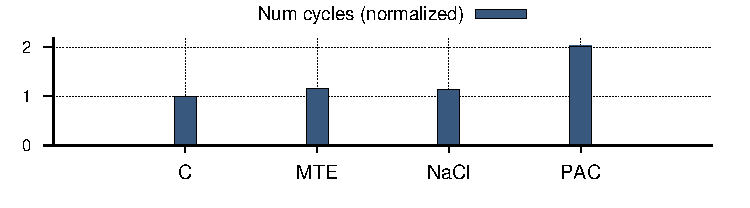
\includegraphics[width=1.0\columnwidth]{figures/ffmpeg-arm.pdf}
\caption{Overhead of FFmpeg (ARM)}
	\label{fig:ffmpeg-arm}
%\vspace{-5mm}
\end{figure}

\begin{figure}[H]
	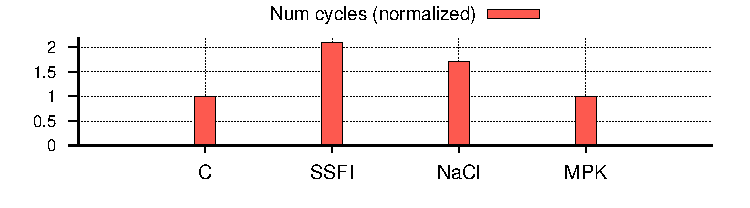
\includegraphics[width=1.0\columnwidth]{figures/ffmpeg-x86.pdf}
\caption{Overhead of FFmpeg (x86)}
	\label{fig:ffmpeg-x86}
%\vspace{-5mm}
\end{figure}